%\newpage
%\section{Заполнение шаблона}
%\begin{itemize}
	%\item Изменить \textbf{config.tex}: имя студента, название предмета и пр. %параметры указаны именно там
	%\item Заполнить \textbf{content.tex} - файл, который будет содержать весь %текст отчёта, от вступления до заключения.
	%\item Добавить используемую литературу (если есть) в \textbf{refs.bib}. Для %удобного поиска источников можно воспользоваться Google Books. Использованные %источники можно указывать с помощью команды \textbf{\\cite\{name\_of\_ref\}}
%\end{itemize}
%Далее представлены различные примеры.

\section{Цель работы}\label{sec:purpose}

Описание цели работы

\section{Задачи, решаемые в лабораторной работе}\label{sec:tasks}

\begin{itemize}
\item[--] Задача 1 [\ref{sec:graphics}]
\item[--] Задача 2
\item[--] Задача 3
\end{itemize}

\section{Теоретическая информация}\label{sec:теоретическая-информация}

Было использовано методическое указание по выполнению лабораторного практикума по основам фотоники.
Исследование кинетических свойств фотохромных стекол~\cite{conlan1983massive}.

\section{Рабочие формулы и исходные данные}\label{sec:initial_data}

Перечень формул

\section{Оборудования и принадлежности}\label{sec:stuff}

Таблица оборудования, их характеристик и возможно subsection со схемами установок
\subsection{Схема установки}\label{subsec:schemes}

\section{Результаты эксперимента}\label{sec:results}

Пишем о результатах эксперимента

\section{Графики}\label{sec:graphics}

\begin{figure}[H]
        \centering
        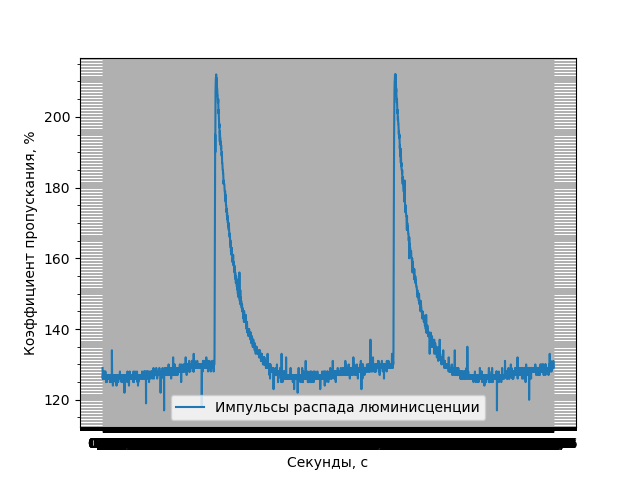
\includegraphics{figures/example}%[width=]
        \caption{Какой-то график}
		\label{fig:someFigure}
\end{figure}

\section{Выводы и анализы результатов}\label{sec:conclution}
В данной работе я измерил интегральную оптическую плотность фотохромного стекла, рассчитал добавочную оптическую плотность и критерий релаксации.
Среди образцов 1--7:
\begin{itemize}
	\item Образец №2 обладает наибольшей степенью потемнения (потемнение наиболее значительно, в сравнении с остальными образцами)
	\item Образец №5 наивысшим критерием релаксации (наиболее быстрое обесцвечивание)
	\item Образец №2 обладает наивысшим показателем оптической плотности (наибольшая степень потемнения)
\end{itemize}
